\chapter{Собственное время, замедление времени и сокращение длины}

Мы часто будем выбирать единицы, в которых скорость света равна $c=1$. В этих единицах год времени и световой год расстояния можно сравнивать непосредственно, и формулы читать гораздо легче. Всякий раз, когда $c$ физически существенна, мы будем возвращать её обратно. Размерностного анализа достаточно, чтобы определить, где она должна стоять.

\section{Галилеева пространственно-временная сетка}

Начнем с доэйнштейновского соотношения между покоящейся системой отсчета и поездом, движущимся со скоростью $v$ вдоль оси $x$:
\begin{align}
x' &= x-vt, & t'&=t.
\label{eq:l4-galilean}
\end{align}
Во втором уравнении содержится ньютоновское предположение об универсальном времени. Все наблюдатели пользуются одними и теми же срезами одновременности, хотя пространственные начала координат движутся друг относительно друга.

Предположим, что нештрихованный наблюдатель стоит у пути, а штрихованный наблюдатель едет в поезде. Начало координат поезда имеет $x'=0$, поэтому его мировая линия в нештрихованных координатах имеет вид
\begin{equation}
x=vt.
\end{equation}
Эта наклонная прямая есть ось $t'$. Напротив, $t'=t$ означает, что все линии постоянного $t'$ — это те же горизонтальные линии, что и линии постоянного $t$.

\begin{figure}[H]
\centering
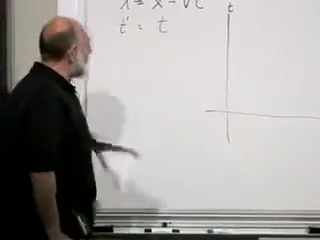
\includegraphics[width=0.72\textwidth]{lecture_04_figure_02.png}
\caption{Галилеево преобразование и исходная сетка $t$-$x$. Движущееся начало координат будет описывать $x=vt$, тогда как обе системы сохраняют общие линии постоянного времени.}
\lectureframe{00:03:06}
\end{figure}

Решая уравнение~\eqref{eq:l4-galilean} относительно нештрихованных координат, получаем
\begin{align}
x&=x'+vt'=x'+vt, & t&=t'.
\end{align}
Обратное преобразование имеет тот же вид, если заменить $v$ на $-v$. Если поезд движется вперед относительно станции, то станция движется назад относительно поезда. Эта взаимность сохраняется и в специальной теории относительности, а вот универсальное время — нет.

\section{Лоренцевская поправка}

Галилеевы преобразования не могут сделать скорость света одинаковой во всех инерциальных системах отсчета. Исправленные соотношения имеют вид, сначала в единицах $c=1$,
\begin{align}
x'&=\frac{x-vt}{\sqrt{1-v^2}}, &
t'&=\frac{t-vx}{\sqrt{1-v^2}}.
\label{eq:l4-lorentz-natural}
\end{align}
После восстановления обычных единиц получаем
\begin{align}
x'&=\frac{x-vt}{\sqrt{1-v^2/c^2}}, &
t'&=\frac{t-vx/c^2}{\sqrt{1-v^2/c^2}}.
\label{eq:l4-lorentz-c}
\end{align}

\begin{figure}[H]
\centering
\includegraphics[width=0.74\textwidth]{lecture_04_figure_05.png}
\caption{Преобразование Лоренца с восстановленными множителями $c$.}
\lectureframe{00:09:10}
\end{figure}

При $v\ll c$ и $v^2/c^2$, и $vx/c^2$ малы в тех условиях, где используется ньютоновская механика. Тогда уравнение~\eqref{eq:l4-lorentz-c} сводится к галилеевскому результату. Теория относительности не отбрасывает ньютоновскую кинематику; она устанавливает область её применимости.

При $v=c$ знаменатель обращается в нуль. Одна инерциальная система отсчета не может двигаться со скоростью света относительно другой инерциальной системы отсчета. Значительно ниже этого предела поправки малы, но вблизи него смешивание $x$ и $t$ становится неизбежным.

Движение выбрано вдоль $x$, поэтому поперечные координаты не меняются:
\begin{equation}
y'=y,\qquad z'=z.
\end{equation}
Один из способов понять, почему, — разместить одинаковые поперечные метровые стержни в поезде и на платформе. Наблюдатель в системе отсчета, промежуточной между двумя данными системами, видит, что стержни сближаются с равными по модулю и противоположными по направлению скоростями. В этой постановке нет ничего, что могло бы сделать один поперечный стержень короче другого.

\section{Преобразования Лоренца вдоль светового конуса}

Уравнение~\eqref{eq:l4-lorentz-natural} можно истолковать геометрически. Сложим два его уравнения:
\begin{align}
t'+x'
&=\frac{(t-vx)+(x-vt)}{\sqrt{1-v^2}}\\
&=(t+x)\frac{1-v}{\sqrt{1-v^2}}\\
&=(t+x)\sqrt{\frac{1-v}{1+v}}.
\label{eq:l4-null-plus}
\end{align}
Вычтем их в обратном порядке:
\begin{align}
t'-x'
&=\frac{(t-vx)-(x-vt)}{\sqrt{1-v^2}}\\
&=(t-x)\frac{1+v}{\sqrt{1-v^2}}\\
&=(t-x)\sqrt{\frac{1+v}{1-v}}.
\label{eq:l4-null-minus}
\end{align}

\begin{figure}[H]
\centering
\includegraphics[width=0.75\textwidth]{lecture_04_figure_06.png}
\caption{Преобразование Лоренца, переписанное через нулевые комбинации
$t+x$ и $t-x$. Их коэффициенты масштабирования взаимно обратны.}
\lectureframe{00:18:45}
\end{figure}

Комбинации $t+x$ и $t-x$ являются координатами вдоль двух светоподобных направлений под $45^\circ$. Буст сжимает одно из этих направлений и растягивает другое с обратным коэффициентом. Он не отклоняет ни одно из них от $45^\circ$. Поэтому световые лучи остаются световыми лучами; такова пространственно-временная картина инвариантности скорости света.

\begin{classroomqa}
\audiencequestion{Наблюдатель промежуточной системы видит симметричный эксперимент, но как из этого следует результат для наблюдателей в поезде и на платформе?\lecturetimestamp{00:20:48}}
\lecturerresponse{Используется еще один факт: совпадение событий инвариантно. Если концы стержней встречаются, то эта встреча представляет собой одно пространственно-временное событие. Любой инерциальный наблюдатель может приписать ему разные координаты, но ни один не может расщепить одно совпадение на два разных места. Вспышки, испускаемые там, где встречаются соответствующие концы, делают эти события операционально обнаружимыми. Симметрия промежуточной системы и инвариантность двух совпадений на концах устанавливают, что поперечные длины одинаковы.}
\end{classroomqa}

\begin{classroomqa}
\audiencequestion{Должен ли велосипедист, представляющий промежуточную систему отсчета, физически находиться в середине между стержнями?\lecturetimestamp{00:22:25}}
\lecturerresponse{Нет. Система отсчета — это целая сеть наблюдателей и часов, а не один глаз в одной точке. Велосипедист может получить вспышки от концов позже и заключить, где они были испущены. Существенно пространственно-временное положение каждого события излучения, а не то, где свет в конечном счете принимается.}
\end{classroomqa}

Сложение скоростей — еще одно следствие того же преобразования, но оно намеренно оставлено до следующей лекции. Наша нынешняя задача — выделить инвариантную величину, которую измеряют движущиеся часы.

\section{Инвариантный интервал}

При повороте обычных декартовых осей величина $x^2+y^2$ не изменяется. Преобразования Лоренца сохраняют другую квадратичную форму. Из уравнения~\eqref{eq:l4-lorentz-natural} получаем
\begin{align}
t'^2-x'^2
&=\frac{(t-vx)^2-(x-vt)^2}{1-v^2}\\
&=\frac{t^2-2vtx+v^2x^2-x^2+2vtx-v^2t^2}{1-v^2}\\
&=t^2-x^2.
\label{eq:l4-interval}
\end{align}
Смешанные члены сокращаются, а в оставшемся числителе содержится общий множитель $1-v^2$.

\begin{figure}[H]
\centering
\includegraphics[width=0.76\textwidth]{lecture_04_figure_07.png}
\caption{Вывод на доске равенства $t'^2-x'^2=t^2-x^2$.}
\lectureframe{00:33:15}
\end{figure}

В трех пространственных измерениях инвариант имеет вид
\begin{equation}
t'^2-x'^2-y'^2-z'^2=t^2-x^2-y^2-z^2
\end{equation}
в единицах $c=1$. В более общем случае для двух событий используются разности координат:
\begin{equation}
\Delta s^2
=c^2\Delta t^2-\Delta x^2-\Delta y^2-\Delta z^2.
\label{eq:l4-spacetime-interval}
\end{equation}
Все инерциальные наблюдатели согласны относительно этого числа, хотя относительно его отдельных временной и пространственных составляющих они не согласны.

\section{Собственное время и движущиеся часы}

Представьте себе решетку покоящихся наблюдателей, часы которых синхронизированы путем обмена световыми сигналами. Их показания определяют координатное время $t$. Теперь пронесем одни ручные часы через эту решетку. Их собственное показание сопровождает их вдоль мировой линии; это показание и есть собственное время.

Для двух временеподобно разделенных событий определим
\begin{equation}
c^2\Delta\tau^2
=c^2\Delta t^2-\Delta x^2-\Delta y^2-\Delta z^2.
\label{eq:l4-proper-time}
\end{equation}
В одном пространственном измерении при $c=1$ это просто
\begin{equation}
\Delta\tau=\sqrt{\Delta t^2-\Delta x^2}.
\end{equation}
Квадратный корень здесь аналогичен формуле для обычного расстояния, но знак минус меняет геометрию.

Имеются три случая:
\begin{align}
\Delta t^2-\Delta x^2 &>0 &&\text{timelike},\\
\Delta t^2-\Delta x^2 &=0 &&\text{lightlike},\\
\Delta t^2-\Delta x^2 &<0 &&\text{spacelike}.
\end{align}
Внутри светового конуса собственное время действительно. На самом конусе, где $x=\pm t$, оно равно нулю, хотя события не обязаны совпадать. Именно такие события может соединять световой луч. Вне конуса разделение пространственноподобно; его лучше описывать действительным собственным расстоянием $\sqrt{\Delta x^2-\Delta t^2}$, чем мнимым временем часов.

\begin{figure}[H]
\centering
\includegraphics[width=0.73\textwidth]{lecture_04_figure_08.png}

\vspace{0.8em}

\begin{tikzpicture}[x=1.0cm,y=1.0cm]
\draw[->] (-3.3,0) -- (3.3,0) node[right] {$x$};
\draw[->] (0,-0.4) -- (0,4.0) node[above] {$t$};
\draw[thick] (0,0) -- (3.0,3.0) node[above right] {$x=t$};
\draw[thick] (0,0) -- (-3.0,3.0) node[above left] {$x=-t$};
\node at (0,2.0) {timelike};
\node at (2.25,1.05) {spacelike};
\node at (-2.25,1.05) {spacelike};
\end{tikzpicture}
\caption{Световой конус на доске и четкая классификация временеподобного,
светоподобного и пространственноподобного разделения.}
\lectureframe{00:38:40}
\end{figure}

Почему формула~\eqref{eq:l4-proper-time} дает показание часов? Для часов, находящихся в покое, $\Delta x=0$, так что $\Delta\tau=\Delta t$. Для равномерно движущихся часов выберем штрихованную систему, в которой эти часы покоятся. Там $\Delta x'=0$, и инвариантность дает
\begin{equation}
\Delta\tau
=\sqrt{\Delta t'^2-\Delta x'^2}
=\Delta t'.
\end{equation}
Следовательно, движущиеся часы отсчитывают собственное время.

\begin{classroomqa}
\audiencequestion{Используются ли ``интервал между событиями'' и ``показание часов'' как два названия одного и того же?\lecturetimestamp{00:44:49}}
\lecturerresponse{Они совпадают, когда идеальные часы движутся по инерции от одного события к другому. Инвариантный интервал — геометрическая величина; разность показаний сопутствующих часов в начальном и конечном событиях дает его физическое измерение. Стационарные координатные часы, как правило, регистрируют иной интервал координатного времени.}
\end{classroomqa}

\section{Замедление времени и одновременность}

Рассмотрим начало движущейся системы отсчета. Его мировая линия задается соотношениями
\begin{equation}
x'=0,\qquad x=vt.
\end{equation}
Та же наклонная прямая является и траекторией движущихся часов, и осью $t'$.

\begin{figure}[H]
\centering
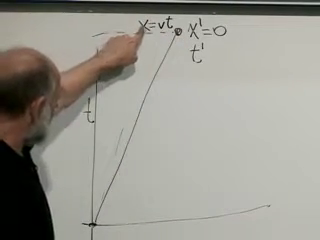
\includegraphics[width=0.72\textwidth]{lecture_04_figure_03.png}
\caption{Движущееся начало координат: $x=vt$, $x'=0$ и ось $t'$ — это три описания одной и той же мировой линии.}
\lectureframe{00:48:18}
\end{figure}

Применим инвариантный интервал между общим началом координат и более поздней точкой на этой мировой линии:
\begin{align}
t'^2-x'^2&=t^2-x^2,\\
t'^2&=t^2-v^2t^2,\\
t'&=t\sqrt{1-v^2}.
\label{eq:l4-time-dilation-natural}
\end{align}
После восстановления $c$ получаем
\begin{equation}
\Delta\tau=\Delta t\sqrt{1-\frac{v^2}{c^2}}
=\frac{\Delta t}{\gamma},
\qquad
\gamma=\frac{1}{\sqrt{1-v^2/c^2}}.
\label{eq:l4-time-dilation}
\end{equation}

\begin{figure}[H]
\centering
\includegraphics[width=0.73\textwidth]{lecture_04_figure_09.png}
\caption{Результат для замедления времени на доске: движущиеся часы отсчитывают
$t'=t\sqrt{1-v^2}$ в единицах, где $c=1$.}
\lectureframe{00:50:45}
\end{figure}

Неподвижный наблюдатель говорит, что движущиеся часы идут медленнее. Принцип взаимности требует, чтобы движущийся наблюдатель говорил то же самое о неподвижных часах. Противоречия нет, потому что эти два описания сравнивают разные пары удалённых событий.

Действительно, постоянное значение $t'$ в уравнении~\eqref{eq:l4-lorentz-natural} удовлетворяет
\begin{equation}
t-vx=\text{constant}.
\label{eq:l4-simultaneity}
\end{equation}
Линии одновременности движущегося наблюдателя наклонены относительно горизонтальных линий $t=\text{constant}$. Каждый наблюдатель считает одновременным свой набор показаний удалённых часов. Если ясно удерживать это различие, взаимное замедление часов оказывается непротиворечивым.

\begin{figure}[H]
\centering
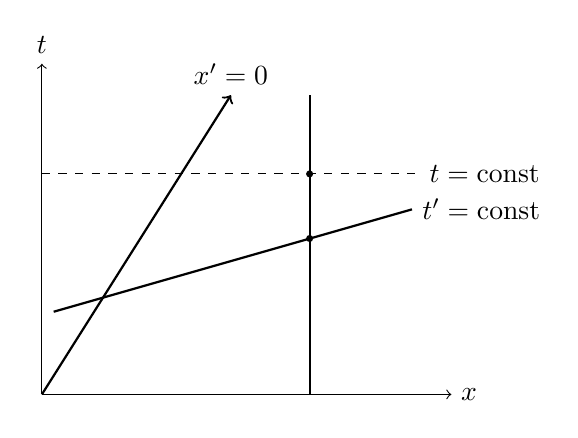
\begin{tikzpicture}[x=1cm,y=1cm]
\draw[->] (0,0) -- (0,4.2) node[above] {$t$};
\draw[->] (0,0) -- (5.2,0) node[right] {$x$};
\draw[thick,->] (0,0) -- (2.4,3.8) node[above] {$x'=0$};
\draw[dashed] (0,2.8) -- (4.8,2.8)
  node[right] {$t=\mathrm{const}$};
\draw[thick] (0.15,1.05) -- (4.7,2.35)
  node[right] {$t'=\mathrm{const}$};
\draw[thick] (3.4,0) -- (3.4,3.8);
\fill (3.4,2.8) circle (0.045);
\fill (3.4,1.98) circle (0.045);
\end{tikzpicture}
\caption{При взаимном замедлении времени сравниваются показания часов на разных срезах одновременности.}
\end{figure}

\section{Пути близнецов}

Два близнеца начинают в одном и том же событии. Один остаётся при $x=0$. Другой удаляется со скоростью $v$, меняет направление и возвращается с той же скоростью. Когда они снова встречаются, они сравнивают все физические процессы, которые могут служить часами: наручные часы, сердцебиение, обмен веществ или само старение.

Пусть каждая половина путешествия занимает координатное время $T$ в домашней системе отсчёта. Собственное время домашнего близнеца равно
\begin{equation}
\tau_{\mathrm{home}}=2T.
\end{equation}
Событие разворота имеет координаты $(vT,T)$. Поэтому первый участок пути путешествующего близнеца даёт вклад
\begin{align}
\tau_{\mathrm{leg}}
&=\sqrt{T^2-v^2T^2}
=T\sqrt{1-v^2}.
\end{align}
Обратный участок даёт такую же величину, следовательно,
\begin{equation}
\tau_{\mathrm{travel}}=2T\sqrt{1-v^2}<2T.
\label{eq:l4-twin}
\end{equation}

\begin{figure}[H]
\centering
\includegraphics[width=0.73\textwidth]{lecture_04_figure_10.png}

\vspace{0.8em}

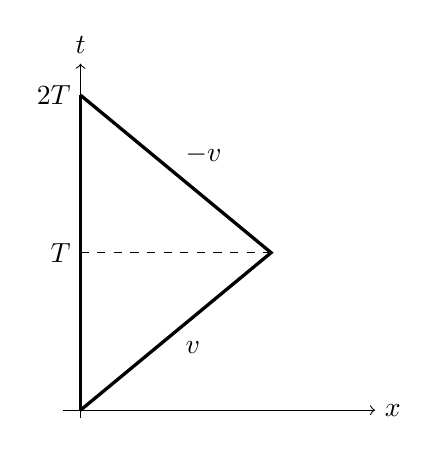
\begin{tikzpicture}[x=1.1cm,y=1cm]
\draw[->] (-0.2,0) -- (3.4,0) node[right] {$x$};
\draw[->] (0,-0.1) -- (0,4.4) node[above] {$t$};
\draw[very thick] (0,0) -- (0,4);
\draw[very thick] (0,0) -- (2.2,2) -- (0,4);
\draw[dashed] (0,2) -- (2.2,2);
\node[left] at (0,2) {$T$};
\node[left] at (0,4) {$2T$};
\node[below right] at (1.1,1.0) {$v$};
\node[above right] at (1.1,3.0) {$-v$};
\end{tikzpicture}
\caption{Мировая линия домашнего близнеца и два участка пути путешествующего. Их собственные времена различны, потому что это разные пути в пространстве-времени.}
\lectureframe{00:59:35}
\end{figure}

В неравенстве возрастов нет противоречия. Траектория путешественника содержит поворот и не связана с прямой домашней траекторией единым преобразованием симметрии между инерциальными системами отсчёта. В обычной евклидовой геометрии прямой маршрут и ломаный маршрут между двумя точками тоже имеют разные длины. Геометрия Минковского меняет местами то, у какого пути интервал больше, но само сравнение остаётся геометрическим.

\section{Ускорение и идеальные часы}

\begin{classroomqa}
\audiencequestion{При развороте физика иная, и путешественник ускоряется. Не делает ли это расчёт по показаниям часов недействительным?
\lecturetimestamp{01:02:19}}
\lecturerresponse{Ускорение реально и помогает выявить асимметрию; не следует от него отмахиваться. Острый угол — лишь идеализированный рисунок, и его можно сгладить, заменив разворотом конечной длительности. Дополнительное физическое предположение состоит в том, что достаточно малые и хорошо устроенные часы нечувствительны к умеренному ускорению и продолжают отсчитывать собственное время. Большие или хрупкие часы могут деформироваться или сломаться, но это недостаток механизма, а не пространственно-временного интервала.}
\end{classroomqa}

Это предположение об идеальных часах не выводится из одного лишь преобразования Лоренца. Его проверяют по поведению реальных часовых механизмов. Атом является гораздо лучшим приближением, чем часы размером в сотни миль, потому что компактный механизм труднее деформировать под действием ускорения или гравитации. Простое упоминание общей теории относительности не устранило бы этой физической проблемы; всё равно пришлось бы знать, как выбранный механизм реагирует на окружающие условия.

\begin{classroomqa}
\audiencequestion{Можно ли свести ускоренную траекторию к коротким интервалам, на которых инерциальный анализ остаётся применимым?\lecturetimestamp{01:09:08}}
\lecturerresponse{Да. Разбейте кривую на короткие, почти прямые отрезки, вычислите собственное время на каждом отрезке и сложите результаты. Это пространственно-временной аналог нахождения длины обычной кривой из многих малых отрезков. В пределе непрерывности,
\[
\tau=\int \sqrt{1-\frac{v(t)^2}{c^2}}\,dt,
\]
для движения в плоском пространстве-времени, описанного в инерциальной системе координат.}
\end{classroomqa}

\section{Что видят близнецы}

Окончательные показания часов можно операционально задать, посылая световые импульсы. Отметьте на обеих мировых линиях интервалы собственного времени по одной секунде и пусть каждый близнец испускает импульс на каждой отметке. На участке удаления импульсы, получаемые от другого близнеца, приходят с большими промежутками. На участке возвращения они приходят плотной группой. Это релятивистский эффект Доплера, непосредственно выраженный на пространственно-временной диаграмме.

\begin{figure}[H]
\centering
\includegraphics[width=0.73\textwidth]{lecture_04_figure_11.png}
\caption{Световые сигналы между домашней мировой линией и мировой линией путешественника. Редкие приходы на участке удаления и сближенные на участке возвращения позволяют учесть каждый испущенный импульс.}
\lectureframe{01:12:55}
\end{figure}

Ни одна система отсчёта в этом рассказе не исчезает. Каждый наблюдатель в конце концов получает все импульсы, испущенные другим, но частота их приёма зависит от относительного движения. Красное смещение на удалении и синее смещение на сближении действуют для двух путей не в течение одинаковых промежутков времени, поэтому подсчёт всех принятых импульсов согласуется со сравнением собственных времён.

\begin{classroomqa}
\audiencequestion{Если возвращающийся путешественник принимает свет, смещённый в синюю сторону, может ли он собрать больше энергии, чем излучил источник?
\lecturetimestamp{01:13:50}}
\lecturerresponse{Для этого вопроса нужны релятивистское определение энергии и её зависимость от системы отсчёта, которые мы ещё не ввели. Это разумный вопрос, но одних лишь координат и подсчёта импульсов недостаточно, чтобы свести энергетический баланс, особенно для ускоренного наблюдателя. Поэтому ответ лучше отложить, а не угадывать.}
\end{classroomqa}

\section{Замкнутое пространственное направление}

\begin{classroomqa}
\audiencequestion{Предположим, что одно пространственное направление компактно. Может ли близнец равномерно двигаться вдоль него, вернуться в исходную точку и вовсе обойтись без ускорения? Что тогда различает близнецов?\lecturetimestamp{01:15:14}}
\lecturerresponse{Пространство следует представлять внутренне как цилиндр, а не как лист, изогнутый внутри большего пространства; радиального ускорения может вовсе не быть. Тем не менее возвращающийся наблюдатель сталкивается с глобальным фактом: одни и те же места повторяются. Это указывает на асимметрию, но полный ответ требует аккуратного рассмотрения специальной теории относительности при таком пространственном отождествлении. Здесь вопрос оставлен открытым, а не закрыт импровизированным ответом.}
\end{classroomqa}

\begin{figure}[H]
\centering
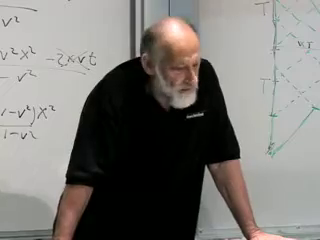
\includegraphics[width=0.72\textwidth]{lecture_04_figure_04.png}

\vspace{0.8em}

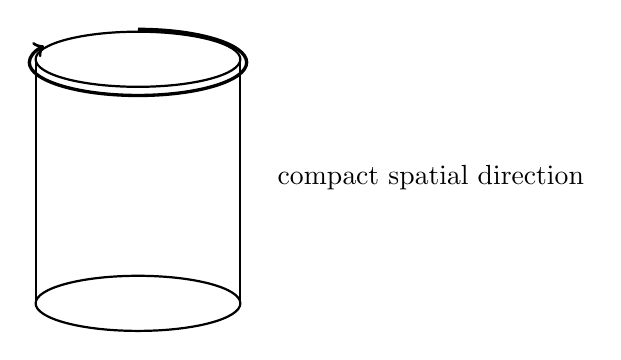
\begin{tikzpicture}[x=1cm,y=1cm]
\draw[thick] (0,0) ellipse (1.3 and 0.35);
\draw[thick] (-1.3,0) -- (-1.3,-3.1);
\draw[thick] (1.3,0) -- (1.3,-3.1);
\draw[thick] (0,-3.1) ellipse (1.3 and 0.35);
\draw[->,very thick] (0.0,0.38) arc (90:-210:1.38 and 0.42);
\node[right] at (1.65,-1.5) {compact spatial direction};
\end{tikzpicture}
\caption{Вопрос о компактном пространстве в том виде, как он нарисован на доске, с чисто внутренне заданным цилиндром. Это вопрос о глобальном отождествлении, а не о движении вокруг цилиндра, вложенного в дополнительное радиальное измерение.}
\lectureframe{01:17:56}
\end{figure}

\section{Длина измеряется на срезе одновременности}

В задаче по специальной теории относительности сначала нарисуйте пространственно-временную картину. Возьмите метровый стержень, покоящийся в нештрихованной системе отсчёта, с концами при $x=0$ и $x=1$. С течением времени оба конца прочерчивают вертикальные мировые линии. Стержень заметает между ними ленту.

Движущийся наблюдатель должен измерить оба конца при одном значении движущегося времени $t'$. Из уравнения~\eqref{eq:l4-simultaneity} следует, что срез, проходящий через начало координат и имеющий $t'=0$, удовлетворяет
\begin{equation}
t=vx
\end{equation}
в единицах $c=1$. Он пересекает правый конец $x=1$ при $t=v$.

\begin{figure}[H]
\centering
\includegraphics[width=0.73\textwidth]{lecture_04_figure_12.png}

\vspace{0.8em}

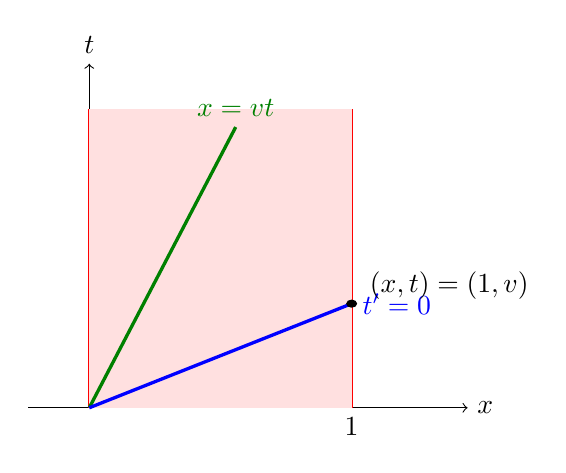
\begin{tikzpicture}[x=1.55cm,y=1.15cm]
\draw[->] (-0.5,0) -- (3.1,0) node[right] {$x$};
\draw[->] (0,0) -- (0,3.8) node[above] {$t$};
\draw[very thick,red] (0,0) -- (0,3.3);
\draw[very thick,red] (2.15,0) -- (2.15,3.3);
\fill[red!12] (0,0) rectangle (2.15,3.3);
\draw[very thick,green!50!black] (0,0) -- (1.2,3.1)
  node[above] {$x=vt$};
\draw[very thick,blue] (0,0) -- (2.15,1.15)
  node[right] {$t'=0$};
\fill (2.15,1.15) circle (0.045);
\node[right] at (2.22,1.35) {$(x,t)=(1,v)$};
\node[below] at (2.15,0) {$1$};
\end{tikzpicture}
\caption{Покоящийся стержень заметает пространственно-временную ленту. Длина, измеряемая движущимся наблюдателем, есть расстояние между его концами на одном срезе $t'=\mathrm{const}$.}
\lectureframe{01:24:20}
\end{figure}

Выбранное разделение концов пространственноподобно, поэтому используем положительную пространственную форму инварианта:
\begin{equation}
x'^2-t'^2=x^2-t^2.
\end{equation}
В выбранном конце $t'=0$, $x=1$ и $t=v$. Следовательно,
\begin{align}
x'^2&=1-v^2,\\
x'&=\sqrt{1-v^2}.
\end{align}
Таким образом, собственная длина $L$ измеряется в движущейся системе как
\begin{equation}
L'=L\sqrt{1-v^2/c^2}=\frac{L}{\gamma}.
\label{eq:l4-length-contraction}
\end{equation}

\begin{figure}[H]
\centering
\includegraphics[width=0.76\textwidth]{lecture_04_figure_13.png}
\caption{Завершённое построение сокращения длины и полученный на доске результат $x'=\sqrt{1-v^2}$ для единичной собственной длины.}
\lectureframe{01:28:10}
\end{figure}

Верно и обратное утверждение: наблюдатель на платформе приписывает меньшую длину продольному метровому стержню в поезде. И снова два наблюдателя выбирают разные одновременные события на концах, поэтому взаимность здесь не ведёт к противоречию.

\section{Вопросы в конце}

\begin{classroomqa}
\audiencequestion{Распространяется ли что-нибудь, кроме света, со скоростью света? В частности, как обстоит дело с гравитацией?\lecturetimestamp{01:29:29}}
\lecturerresponse{Общая теория относительности предсказывает гравитационные волны, распространяющиеся со скоростью $c$. Во время этой лекции свидетельства были косвенными и исходили от таких систем, как двойные пульсары; гравитационные волны ещё не были непосредственно обнаружены.\editorialnote{После этой лекции 2006 года экспериментальная ситуация изменилась. LIGO непосредственно зарегистрировал GW150914 в 2015 году, а совместное наблюдение GW170817 и его электромагнитного аналога в 2017 году показало, что скорости распространения гравитации и света совпадают с точностью до нескольких частей на $10^{15}$. См. \url{https://ligo.org/detections/gw150914/} и \url{https://doi.org/10.1103/PhysRevLett.119.251302}.}}
\end{classroomqa}

\begin{classroomqa}
\audiencequestion{Может ли астронавт преодолеть расстояние во много световых лет за собственное время, меньшее, чем это расстояние, выраженное в световых годах? Означало бы это движение быстрее света?\lecturetimestamp{01:30:38}}
\lecturerresponse{Собственное время астронавта равно $\sqrt{\Delta t^2-\Delta x^2}$, что меньше координатного времени $\Delta t$. В инерциальной системе астронавта расстояние между звёздами сокращено по Лоренцу. Звёзды движутся со скоростью $-v$, а не быстрее света; просто нужно пересечь меньшее, сокращённое расстояние.}
\end{classroomqa}

Если астронавт начинает из состояния покоя и разгоняется, описание меняется при переходе от одной мгновенно сопутствующей инерциальной системы отсчёта к другой. При этом расстояние, приписываемое звёздам, может меняться. Нельзя применить одно фиксированное преобразование Лоренца ко всей истории с ускорением, но полное собственное время всё равно получается суммированием вкладов вдоль мировой линии. То же самое относится и к реалистичному близнецу, который стартует, разворачивается и тормозит, а не рождается уже на крейсерской скорости.

\begin{classroomqa}
\audiencequestion{Вызваны ли эти парадоксы тем, что мы считаем время чем-то особым? Должны ли мы называть его четвёртым измерением?\lecturetimestamp{01:36:43}}
\lecturerresponse{Необязательно начинать с лозунга о том, что время — четвёртое измерение. Само преобразование Лоренца приводит к смешению пространства и времени, а интервал $t^2-x^2-y^2-z^2$ рассматривает их как части единой геометрии, в которой у времени и пространства разные знаки. При малых скоростях это смешение становится пренебрежимо малым, и возвращается привычная ньютоновская интуиция. Однако при релятивистских скоростях пространство и время нельзя считать принципиально независимыми друг от друга.}
\end{classroomqa}

Поэтому замедление времени, сокращение длины, сравнение близнецов и сокращённое время в пути не являются отдельными уловками. Всё это вытекает из трёх привычек: определять сравниваемые события, изображать их геометрию в пространстве-времени и использовать инвариантный интервал.